\documentclass[aps,prd,amssymb,amsmath,amsfonts,superscriptaddress,
floatfix ,preprintnumbers,altaffilletter]{revtex4}

\usepackage{epsfig}
\usepackage{graphics}
\usepackage{graphicx}
\usepackage{amsmath,amssymb,mathrsfs}
\usepackage{amsfonts}
\usepackage{color}
\usepackage{wasysym}
\usepackage{times}
\usepackage{mathptmx}
\usepackage{gensymb}
%\usepackage{fullpage}
\usepackage{appendix}
%\usepackage{fontenc}
\usepackage{listings}
%\usepackage[utf8]{inputenc}
%\usepackage{authblk}
\usepackage{listings}
\usepackage{url}

%%%%%Some new commands%%%%%%%%%%%%%%%%%
% Macros for text changes
\newcommand{\red}{\textcolor{red}}
\newcommand{\patricia}[1]{\textcolor{blue}{\textit{Patricia: #1}}}
\newcommand{\ian}[1]{\textcolor{blue}{\textit{Ian: #1}}}

\newcommand{\AEI}{Max Planck Institute for Gravitational Physics (Albert-Einstein-Institute), Am M\"uhlenberg 1, Potsdam-Golm, 14476, Germany}
\newcommand{\Ligo}{LIGO Laboratory, California Institute of Technology, MS 100-36, Pasadena, California 91125, USA}
\newcommand{\TAPIR}{Theoretical Astrophysics, Walter Burke Institute for Theoretical Physics, California Institute of Technology, Pasadena, California 91125, USA}
\newcommand{\CITA}{Canadian Institute for Theoretical
    Astrophysics, 60 St.~George Street, University of Toronto,
    Toronto, ON M5S 3H8, Canada}
%%%%%%%%%%%%%%%%%%%%%%%%%%%%%%%%%

% SCIENCE MACROS
\newcommand{\ExNR}{\hat e_x}
\newcommand{\EyNR}{\hat e_y}
\newcommand{\EzNR}{\hat e_z}

\newcommand{\tNR}{\theta}
\newcommand{\pNR}{\phi}

%\newcommand{\ErNR}{{\hat e_{r,\rm NR}{}}}
%\newcommand{\EtNR}{{\hat e_{\theta\,\rm NR}{}}}
%\newcommand{\EpNR}{{\hat e_{\phi\,\rm NR}{}}}
\newcommand{\ErNR}{{\hat r}}
\newcommand{\EtNR}{{\hat\theta}}
\newcommand{\EpNR}{{\hat\phi}}

\newcommand{\hpNR}{h_+^{\rm NR}}
\newcommand{\hcNR}{h_{\times}^{\rm NR}}
\newcommand{\nNR}{\hat{n}}

\newcommand{\lNR}{\hat L}

\newcommand{\tGW}{t_{\rm GW}}

%%%%%%%%%%%%%%%%%%%%%%%%%%%%%%%%%%%%%%%%%%%%%%%%%%%%%%%%%%%%%%%%
% SOURCE FRAME

\newcommand{\ExS}{{{\hat x}}}
\newcommand{\EyS}{{{\hat y}}}
\newcommand{\EzS}{{{\hat z}}}

%%%%%%%%%%%%%%%%%%%%%%%%%%%%%%%%%%%%%%%%%%%%%%%%%%%%%%%%%%%%%%%%
% WAVE FRAME

\newcommand{\ExW}{\hat X}
\newcommand{\EyW}{\hat Y}
\newcommand{\EzW}{\hat Z}
\newcommand{\hpW}{h_+^{\rm W}}
\newcommand{\hcW}{h_\times^{\rm W}}


%%%%%%%%%%%%%%%%%%%%%%%%%%%%%%%%%%%%%%%%%%%%%%%%%%%%%%%%%%%%%%%%
% MORE SYMBOLS
\newcommand{\incl}{i}  %  inclination
\newcommand{\phiRef}{\Phi} % ``LAL-phase'' in orbital plane
\newcommand{\meanAnomaly}{\delta} % mean anomaly at reference time
\newcommand{\equalref}{\overset{\rm ref}{=}}

%%%%%%%%%%%%%%%%%%%%%%%%%%%%%%%%%%%%%%%%%%%%%%%%%%%%%%%%%%%%%%%%
%%%%%%%%%%
\begin{document}
%%%%%%%%%%

\title{Numerical Relativity Injection Infrastructure}

\author{Patricia Schmidt}
\affiliation{\Ligo}
\affiliation{\TAPIR}

\author{Ian W. Harry}
\affiliation{\AEI}

\author{Harald P. Pfeiffer}
\affiliation{\AEI}
\affiliation{\CITA}

\date{\today}

\begin{flushright}
LIGO-T1500606-v2
\end{flushright}

%%%%%%%%%%%%%%%
\begin{abstract}
\label{sec:abs}
%%%%%%%%%%%%%%%
This document describes the new standardised NR injection infrastructure in the LIGO Algorithms Library (LAL), 
which henceforth allows for the usage of Numerical Relativity (NR) waveforms as a discrete waveform approximant
in LAL. With this new interface, NR waveforms provided in the appropriate format can directly be
used as mock GW signals (``injections'') for LIGO data analyses, which include parameter estimation, searches, hardware
injections etc. The interface handles higher-order modes making them directly accessible to LIGO analyses for
the very first time. The NR injection infrastructure also takes care of waveform frame conventions and transforms the NR
data into the correct LAL frame. 
\end{abstract}

%%%%%%%%%%%%%%%
\maketitle 

%%%%%%%%%%%%%%%
\section{Introduction}
\label{sec:intro}
%%%%%%%%%%%%%%%
Recently, LIGO has reported the first detection of gravitational waves (GW) from a merging binary black hole system~\cite{Abbott:2016blz}.
Such coalescing compact binaries are prime sources for the ground-bases interferometric GW detectors and play a critical role in LIGO data analysis. Whilst for low-mass systems only the early part of the binary evolution, the inspiral, is accessible to LIGO, for high-mass systems 
also the later stages, in particular the merger and ringdown of the final black, are visible in LIGO's sensitivity band. 

During the early part of the binary coalescence, the emitted gravitational waveforms are accurately described by an
analytic post-Newtonian expansion of the Einstein field equations~\cite{lrr-2014-2}. 
To obtain the waveforms for the final stages, the full non-linear solutions
of the field equations are required, which are provided by Numerical Relativity (NR) (see for example~\cite{Centrella:2010mx} for an overview).
Regarding the usage of NR waveforms for LIGO data analysis, so far, NR merger waveforms have predominantly been used to calibrate the merger-ringdown section of analytic waveform models which describe the complete inspiral-merger-ringdown (IMR) signal~\cite{Khan:2015jqa, Taracchini:2013rva}, to test such models against independent NR waveforms not used in the construction and to determine the physical properties of the remnant black hole~\cite{Healy:2014yta}.

In the Advanced detector era, however, we want to be able to directly use NR waveforms in gravitational-wave searches
and parameter estimation, to test General Relativity and to assess the systematics of analytic waveforms models within
a uniform framework. 
This is now possible with the recently implemented  simple infrastructure, which allows for the treatment of
NR waveforms as a ``discrete'' waveform approximant provided the NR data are available in a \emph{specific format}. 

In previous efforts, BBH hybrid waveforms constructed by combining a PN inspiral with an NR merger-ringdown 
waveform, have been used in LIGO data analysis and parameter estimation in the NINJA and NINJA-2 projects~\cite{Aylott:2009ya, Aasi:2014tra}. These hybrids only contained the dominant harmonics, the $(\ell, |m|) =(2,2)$ modes, and required the NR waveforms to be linearly interpolated and resampled at uniform times for a given sampling rate $f_s$. In the NINJA framework, the resampling was performed 
 \emph{before} inserting the total mass scale, resulting in very memory-intensive operations, since the finest $\Delta t$ for a given $f_s$ is determined by the highest total mass one wants to be able to resolve.
  
The new infrastructure handles this differently, in the following way: Firstly, since it naturally handles higher-order modes, it uses a highly compressed data format to represent the NR data to reduce the storage requirements and reduce I/O time. 
Secondly, the compressed NR data are interpolated using 1D spline interpolation, and the resulting interpolants are evaluated \emph{after} the mass scale has been inserted. This avoids high-memory operations and also bypasses the need to store unnecessarily large data files.
The new injection infrastructure fully implemented in LAL and is intended to supersede any previously used NR modules.

The remainder of this technical document is organised as follows: In Sec. \ref{sec:format} we provide a brief summary
of the NR data format and metadata required as input. In Sec. \ref{sec:gen} we describe the basics of the waveform generation code and give explicit examples of how the NR waveforms are evaluated in lalsimulation/pycbc. Sec. \ref{sec:coordinates} details the frame transformations between the NR simulation frame and the LAL wave frame. We highlight caveats and desired future improvements in Sec.~\ref{sec:discussion}.

%%%%%%%%%%%%%%%
\section{Waveform format}
\label{sec:format}
%%%%%%%%%%%%%%%
In Numerical Relativity one solves for the complete space-time of the binary system. For data analysis
purposes however, one requires the gravitational-wave strain $h(t)$ far from the source. The relevant numerical quantity
is the metric perturbation $h^{TT}_{ij}$ as computed in the transverse-traceless gauge (TT). 

There are different way of computing the metric perturbation from a numerical evolution. The most common methods include
the use of the complex Weyl scalar $\Psi_4$, which is related to the metric perturbation via two time derivatives, or the
Regge-Wheeler-Zerilli formalism, which computes the metric perturbation in the wave-zone as a perturbation of the Schwarzschild
spacetime. 

In the TT gauge, the metric perturbation
has two independent real polarisations, $h_+$ and $h_\times$, which can be written as a complex strain by
\begin{equation}
\label{ }
h = h_+ - i h_\times \in \mathbb{C},
\end{equation}
where $h_+, h_\times \in \mathbb{R}$.

Let $(t,x,y,z)$ be a Cartesian coordinate system in the wave-zone, which is related to the polar coordinates $(r, \theta, \phi)$ by the standard means. In this coordinate system, the metric perturbation is commonly decomposed into \emph{modes}
in a basis of spin-weighted spherical harmonics, ${}^{-2}Y_{\ell m}$, of spin weight $s=-2$, where the GW propagation direction is
the radial unit vector r.
For any point $(\theta, \phi)$ on the unit sphere, the GW strain can then be shown to take the following form:
\begin{equation}
\label{ }
h^\mathrm{NR}(t; \theta, \phi) = h^\mathrm{NR}_+ - i h^\mathrm{NR}_\times = \sum_{\ell=2}^\infty \sum_{m=-\ell}^{\ell} H_{\ell m}(t) {}^{-2}Y_{\ell m}(\theta,\phi).
\end{equation}
As for any wave, we can also write each NR gravitational-wave mode $H_{\ell m}$ as an amplitude $A_{\ell m}$ and a phase
$\Phi_{\ell m}$,
\begin{equation}
\label{ }
H_{\ell m}(t) = A_{\ell m}(t)e^{i\Phi_{\ell m}(t)}.
\end{equation}
The amplitude of each mode is its complex norm, the phase is the unwrapped argument of the complex time series $h_{\ell m}$. 

%%%%%%%%%%%%%%%
\subsection{Spline Compression}
\label{sec:spline}
%%%%%%%%%%%%%%%
Gravitational waveforms for LIGO data analysis purposes require uniform sampling in time for a given sampling frequency $f_s$.
NR datasets however, are commonly not uniformly sampled and if they are, the sampling interval $dt$ may not necessarily
correspond to the one required by data analysis tools. 
It is therefore unavoidable to interpolate the NR data such that for any total
mass M and sampling rate the NR waveforms can be resampled accordingly. Whilst the NR data could simply be interpolated as
they are, we choose to reduce the data by performing 1D spline compression on the NR data~\cite{Galley:2016aa}. This is a particular advantage for long simulations or hybrid PN-NR data, but also significantly reduces the storage and I/O for pure NR data. It is mandatory that the NR data files are provided in the correct compressed file format, which is as follows: \\
\\The 1D spline compression is performed separately for each mode amplitude $A_{\ell m}$ and phase $\Phi_{\ell m}$. The compression is
achieved by applying a greedy algorithm to the NR data, which selects the near-optimal points to construct a univariate spline interpolant
with a specified global accuracy. By default, the interpolants are constructed using fifth degree polynomials and a tolerance of $10^{-6}$,
i.e. if the spline is evaluated at the discrete times $t_i$ of the NR data, the original NR values are recovered with an error smaller than the
specified tolerance. For a detailed description of this method and the accuracy of the obtained interpolants, we refer the reader to~\cite{Galley:2016aa}. The spline compression is performed using the publicly available python package ``romSpline'' by Chad R. Galley~\cite{romspline}. \\
\\The spline interpolants for each amplitude and phase are obtained via \texttt{romSpline.ReducedOrderSpline()} as follows:
\begin{lstlisting}
import romSpline
spline = romSpline.ReducedOrderSpline(time_data, amplitude/phase_data, verbose=False)
spline.write('filename.h5')
\end{lstlisting}
Note: a newer version of romSpline now also allows to pass a group descriptor, i.e. writing to file as intermediate step may be avoided.

Once the spline interpolants have been obtained, they have to be stored as individual groups in a \emph{single HDF5 file} with the following mandatory group naming conventions: 
\begin{itemize}
  \item Amplitude group: \textbf{amp\textunderscore l\#1\textunderscore m\#2}
  \item Phase group: \textbf{phase\textunderscore  l\#1\textunderscore m\#2},
\end{itemize}
where (\#1, \#2) are placeholders for $(\ell, m)$, e.g., for $(\ell=2, m=-2)$ the naming convention is phase\textunderscore l2\textunderscore m-2 and 
amp\textunderscore l2\textunderscore m-2. \\
\\Pure NR data without a hybridised PN inspiral need to have the initial \emph{junk radiation} removed before the spline interpolants are constructed but no tapering should be applied at the beginning or end of the waveform data. Following the LAL waveform convention, the waveforms also need to be aligned such that the peak of the waveform occurs at $t_\mathrm{peak}=0$ before constructing the interpolants. In addition to the amplitude and phase groups, we highly recommend to also include the NR times as a group in the HDF5 file. 

%%%%%%%%%%%%%%%
\subsection{Metadata}
\label{sec:meta}
%%%%%%%%%%%%%%%
The metadata format is adapted from the original NINJA-2 metadata format~\cite{Brown:2007jx}, and whilst then metadata were stored an additional text file, it is now mandatory that each HDF5 contains a \emph{minimal} set of metadata stored as \emph{attributes} of the HDF5 file. 
If a metadata text file exists, however, we recommend that it is additionally included in the HDF5 file.\\
\\In the current implementation, the required metadata which are time-dependent (see list below) have to contain the values associated with the first entry in the stored time series. For pure NR data, since the junk radiation has to be removed, these are \emph{not} the initial data of the simulation. We refer to this very first data point stored in the HDF5 file as the \emph{beginning} of the waveform data. Source frame dependent metadata should be given in the NR simulation frame. \\
\\The required metadata attributes are the following:
\begin{itemize}
\item {[}'NR-group'{]}: string to identify the NR group/code
\item {[}'type'{]}: keyword description of the simulation. Allowed values are: aligned-spins, non-spinning, precessing.
\item{[}'name'{]}: alternative simulation name or internal simulation identifier
\item{[}'object1'{]}: keyword description to identify the object type. Allowed values are: BH, NS
\item {[}'object2'{]}: keyword description to identify the object type. Allowed values are: BH, NS
\item{[}'mass1'{]}: mass of the heavier object; if both objects are 'BH', the unit of mass is arbitrary. If at least one object is a NS, then the unit is solar masses $M_\odot$.
\item{[}'mass2'{]}: mass of the lighter object; if both objects are 'BH', the unit of mass is arbitrary. If at least one object is a NS, then the unit is solar masses $M_\odot$.
\item{[}'eta'{]}: the symmetric mass ratio of the simulation
\item{[}'spin1x'{]}: x-component of the dimensionless spin of the heavier object
\item{[}'spin1y'{]}: y-component of the dimensionless spin of the heavier object 
\item{[}'spin1z'{]}: z-component of the dimensionless spin of the heavier object
\item{[}'spin2x'{]}: x-component of the dimensionless spin of the lighter object
\item{[}'spin2y'{]}: y-component of the dimensionless spin of the lighter object 
\item{[}'spin2z'{]}: z-component of the dimensionless spin of the lighter object
\item{[}'LNhatx'{]}: x-component of the orbital angular momentum unit vector
\item{[}'LNhaty'{]}: y-component of the orbital angular momentum unit vector
\item{[}'LNhatz'{]}: z-component of the orbital angular momentum unit vector
\item{[}'nhatx'{]}: x-component of the orbital separation unit vector
\item{[}'nhaty'{]}: y-component of the orbital separation unit vector
\item{[}'nhatz'{]}: z-component of the orbital separation unit vector
\item{[}'f\textunderscore lower\textunderscore at\textunderscore 1MSUN'{]}: frequency of the $(2,2)$-mode in Hz at the beginning of the waveform scaled to 1 solar mass
\end{itemize}
To reduce potential ambiguities, we further recommend adding the following  additional metadata:
\begin{itemize}
\item{[}'eccentricity'{]}: eccentricity parameter of the simulation
\item {[}'mean\textunderscore anomaly'{]}: mean anomaly at the beginning of the waveform (cf. Eq.~\ref{eq:anomaly}).
\item{[}'PN\textunderscore approximant'{]}: string identifier for the inspiral if hybrid data are stored
\end{itemize}

%%%%%%%%%%%%%%%
\section{NR waveform evaluation in LAL}
\label{sec:gen}
%%%%%%%%%%%%%%%
Once the HDF5 file has been provided, the NR waveforms can be evaluated through the standard waveform interfaces \texttt{ChooseTDWaveform()} in LAL and \texttt{get\textunderscore td\textunderscore waveform()} in pyCBC~\cite{Canton:2014ena}. The approximant name is ``NR\textunderscore hdf5''. 
The spline data are read from file and evaluated for the desired extrinsic parameters. The intrinsic parameters in NR simulations are fixed, internal checks on the mass ratio and the spin components are performed to guarantee the consistency between the values passed in the waveform generation call and metadata values. The waveform generator requires the input spin values to be defined as given in Eqn.~(\ref{eq:SpinConsistency}). In general, these are different to the values of the spin metadata and need to be computed using the metadata for the spins, the orbital angular momentum and the orbital separation.\\
\\For a given starting frequency and total mass, a time array is allocated based on an estimate of the waveform length. We use the LAL function 
\texttt{SimIMRSEOBNRv2ChirpTimeSingleSpin()} to estimate the waveform length with an additional leverage of 10\%. If the NR waveforms are not long enough for a given total mass and starting frequency, the generation is aborted. From the estimated length and the desired sampling rate, the discrete time series for the spline evaluation is
determined.\\

To construct the NR GW polarisations $h^\mathrm{NR}_+$ and $h^\mathrm{NR}_\times$, the splines for each amplitude and phase are evaluated at the points of the discrete time times, weighted by the ${}^{-2}Y_{lm}$, and summed up accordingly:
\begin{align}
\label{}
    \mathrm{Re}(H_{\ell m}) &= A_{\ell m} \cos(\Phi_{\ell m}),   \\
    \mathrm{Im}(H_{\ell m}) &= A_{\ell m} \sin(\Phi_{\ell m}),   \\
    h^\mathrm{NR}_+ &= \sum_{\ell, m} \mathrm{Re}(H_{\ell m}) \mathrm{Re}({}^{-2}Y_{\ell m}) - \mathrm{Im}(H_{\ell m}) \mathrm{Im}({}^{-2}Y_{\ell m}), \\
    h^\mathrm{NR}_\times &= \sum_{\ell, m} -\mathrm{Re}(H_{\ell m}) \mathrm{Im}({}^{-2}Y_{\ell m}) - \mathrm{Im}(H_{\ell m}) \mathrm{Re}({}^{-2}Y_{\ell m}).
\end{align}
Note that all waveform modes $(\ell, m)$ present in the HDF5 file are used
to compute the two polarisations. The algorithm will incorporate any mode between $\ell =2$ and $\ell =8$ if present in the
HDF5 file but at least the $(\ell=2, m=2)$ has to be present in the NR data file. \\
\\
The compressed NR data files do not store the splines themselves, but the knots, errors, the polynomial degree etc. In the pyCBC implementation,
the splines are constructed from the HDF5 file via the python function \texttt{UnivariateSpline}, in the LAL implementation regular GSL interpolation
is performed. Fig.~\ref{fig:waveforms} shows an example comparison between NR waveforms obtained using the pyCBC and the LAL waveform generators. The mismatch
between the waveforms is less than $10^{-7}$. This is consistent with the level of disagreement expected due to the different numerical interpolation
routines. \\
The source code can be found in
\begin{lstlisting}
lalsuite/lalsimulation/src/LALSimIMRNRWaveforms.c  
\end{lstlisting}

%%%%%%%%%%
\subsection{Examples}
%%%%%%%%%%
There are a variety of different ways to generate waveforms using LIGO data analysis software. Here, we give two explicit examples
for function calls in python: The first example uses the pyCBC implementation, the second one uses the SWIG-wrapped version of 
lalsimulation. 

\begin{enumerate}
  \item Using the pyCBC waveform interface \texttt{get\textunderscore td\textunderscore waveform()} :\\
\begin{lstlisting}
from pycbc.waveform import get_td_waveform 

hp, hc = get_td_waveform(approximant='NR_hdf5', 
                         numrel_data='/PATH/TO/HDF5',
                         mass1, mass2,
                         spin1x, spin1y, spin1z,
                         spin2x, spin2y, spin2z, 
                         delta_t, f_lower, f_ref,
                         inclination, distance, 
                         coa_phase)
\end{lstlisting}

\item Using the implementation in lalsimulation through SWIG:\\
\begin{lstlisting}[mathescape=true]
import lalsimulation as lalsim

flags = lalsim.SimInspiralCreateWaveformFlags()

lalsim.SimInspiralSetNumrelData(flags,'/PATH/TO/HDF5')

hp, hc = lalsim.SimInspiralChooseTDWaveform(phiRef, 
              deltaT, m1 * MSUN_SI, m2 * MSUN_SI, 
              s1x, s1y, s1z,
              s2x, s2y, s2z, 
              fStart, fRef, 
              distance, inclination,
              $\lambda_1=0$, $\lambda_2=0$, 
              flags, nonGRparams=None, 
              amplitudeO=-1, phaseO=-1, 
              approximant=lalsim.NR_hdf5),
\end{lstlisting}
where $\lambda_1$ denote the tidal deformation parameters, which vanish in the case of black holes. 
\end{enumerate}
Fig.~\ref{fig:waveforms} shows the two waveform polarizations $h_+$ and $h_{\times}$ for the binary black hole hole case simulated in case 
SXS:BBH:0019 from the publicly available SXS catalogue~\cite{Mroue:2013xna} for a total mass of 50 $\mathrm{M}_\odot$. The dimensionless spins for this simulation are
$\vec{\chi}_1=(0,0,-0.5)$ and $\vec{\chi}_2=(0,0,0.499)$ and the component masses are $m_1=30.01360$ and $m_2=20.00954$.
As extrinsic parameters, we choose the following: distance=100Mpc, inclination=0.4rad, deltaT=1.0/16384, fStart=fRef=18.88Hz. We do not alter
the reference phase but instead pass the metadata value stored in the HDF5 file. We have obtained those polarizations via the lalsimulation interface and also via the test verification code in pycbc. The match between the waveforms obtained from the two numerical implementations is $\mathcal{M}=0.999999999341$.
\begin{figure}
\begin{center}
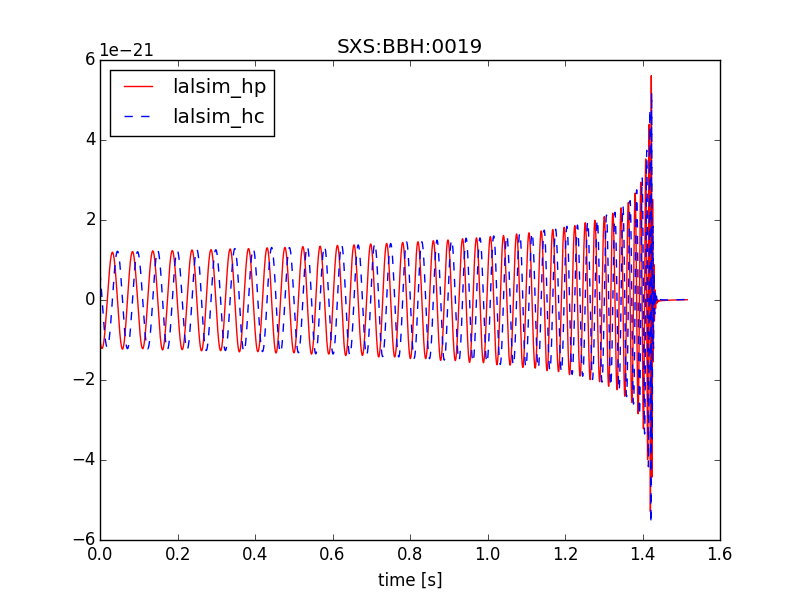
\includegraphics[width=80mm]{lalsim_TD_0019.png}
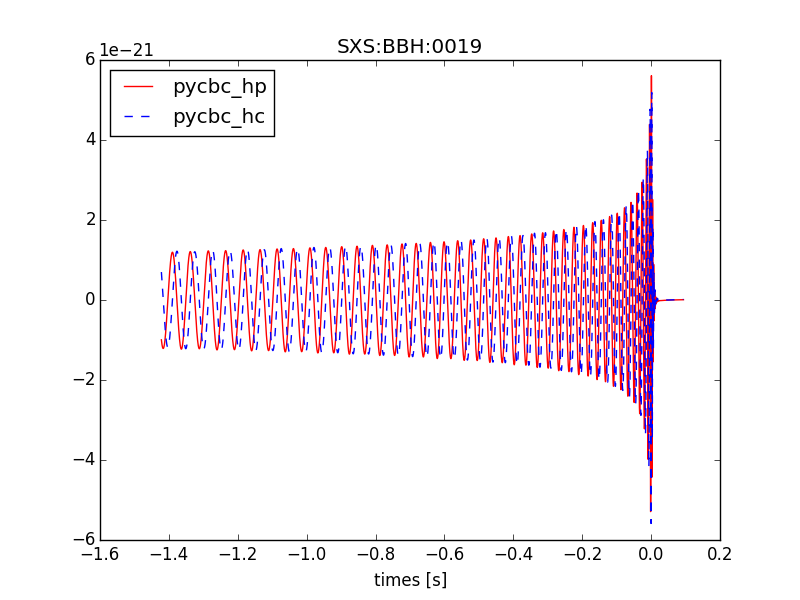
\includegraphics[width=80mm]{pycbc_TD_0019.png}
\caption{\red{Those need to be replaced with updated version.} The waveform polarizations $h_+$(solid, red) and $h_\times$(dashed, blue) of the publicly available SXS waveform SXS:BBH:0019 
generated via the waveform interface in lalsimulation (left panel) and in pyCBC (right panel).}
\label{fig:waveforms}
\end{center}
\end{figure}

%%%%%%%%%%%%%%%%%%%%%%%%%%%%%%%%%%%%%%%%%%%%%%%%%%%%
% Incorporate Harald's document here:
%%%%%%%%%%%%%%%%%%%%%%%%%%%%%%%%%%%%%%%%%%%%%%%%%%%%%%%%%%%%%%%%
\section{LAL coordinate frames for precessing binaries and NR injections}
\label{sec:coordinates}
%%%%%%%%%%%%%%%%%%%%%%%%%%%%%%%%%%%%%%%%%%%%%%%%%%%%%%%%%%%%%%%%

\subsubsection{Executive summary: changes of conventions}

In recent discussions, it became apparent that current LAL conventions
to specify precessing binary compact objects are not ideal: (i) The
phase-angle {\tt phiRef} couples specification of the line-of-sight to
Earth with specification of spin components {\tt S1x, S1y, S1z, S2x,
  S2y, S2z}.  To compute waveforms for the \emph{identical} CBC system
viewed from different directions, one may have to specifiy different
values for the in-plane spin-components {\tt S1x, S1y, S2x, S2y}.
(ii) Several existing waveform models do not conform to the current
LAL convention, already implementing the improvements suggested in this note.

Concretely, it is suggested to specify spin-components in a geometric
way based on the angular momentum $\lNR$ and line connecting body 2 to
body 1, $\nNR$:
\begin{align}
  \mbox{\tt S1x}&\equalref \vec\chi_1\cdot\nNR,\\
  \mbox{\tt S1y}&\equalref \vec\chi_1\cdot (\lNR\times\nNR),\\
  \mbox{\tt S1z}&\equalref \vec\chi_1\cdot\lNR,
\end{align}
(and similarly for the second body).  The symbol $\equalref$ indicates
that equality only holds at the reference time, as spins generically
precess during an inspiral.

Furthermore, it is suggested to specify
orientation of eccentric orbits through the angles
\begin{align}
  \mbox{\tt phiRef} = \phiRef &\equalref \angle(\nNR, \mbox{line-of-ascending-node}),\\
  \mbox{\tt mean\_anomaly}= \delta.& %\equalref\angle(\nNR, \mbox{direction-of-periapse}).
  \end{align}


\subsubsection{Motivation \& benefits of new conventions}

Quite generally waveform modeling requires at least two coordinate
systems, a ``source-frame'' in which it is convenient to specify
properties of the source of gravitational waves, and a ``wave-frame''
which is adopted to wave-propagation to detectors on Earth.
Furthermore, numerical relativity data is specified in whatever
coordinates are employed during the numerical evolution, generally
resulting in a third coordinate system.

This note defines coordinate frames for use in LAL.  Specifically, we
achieve:
\begin{enumerate}
  \item Identification of a set of intrinsic parameters that fully
    describe the dynamics of a binary on an eccentric orbit,
    defined solely in terms of the source-frame (i.e. independent of
    the wave-frame).
  \item Identification of three angles that describe the
    transformation between source- and wave-frame, which are
    independent of the intrinsic parameters.
  \item Identification of parameters describing the orbital phase and
    periapsis location, which have a convenient circular-orbit limit:
    As the eccentricity tends to zero, one of the two phase-parameters
    reduces to the standard orbital phase for circular orbits, whereas
    the other becomes irrelevant.
  \item Identities that relate the basis-vectors in the source-frame to the
    wave-frame (and vice versa).  These identities are written in
    vectorial form and are valid in any coordinate system.
\end{enumerate}

The orthogonal decomposition into intrinsic and extrinsic parameters
(points 1 and 2) allows to change the direction at which a binary is
viewed (i.e. the wave-frame), without having to adjust the parameters
that determine the intrinsic dynamics.  Point 3 prepares the ground
for easy extension to eccentric waveforms.
Point 4 is of particular relevance when translating NR data into
LAL-conventions: Evaluating the vector identities in the NR-coordinate
system, yields immediately the relation between NR coordinates and
wave-frame.


\subsubsection{NR waveform injections}

NR data is assumed to be supplied in the data-format defined
in~\cite{Brown:2007jx}, and so it needs to be transformed into the LAL
wave-frame.  For a given reference time, an entire NR data-set could
in principle be transformed into the LAL frame by suitable
transformations of each $H_{\ell m}$-mode.  Applying such a rotation
on the NR-data as a one-time pre-processing step before using it for
injections suffers from two disadvantages:

First, the person who prepares the NR-data for LAL-use must perform
the rotation, and must do so correctly. Since NR data is prepared
separately by several NR groups, this opens the possibility of
introducing errors in this step.  Second, for precessing systems, the
orbital angular momentum $\lNR$ precesses.  Therefore, pre-rotating
the NR-data locks in the reference point, and one would need to
generate a new pre-rotated NR-data for a different reference point.
Since NR data is in geometric units, the NR-data would have to be
separately rotated whenever the total mass of an injection changes.

To avoid both disadvantages, it is proposed to leave the NR-data in
its original frame.  Instead, the transformations betweeen the
LAL-convention and the NR-data are applied \emph{at use} during the
call to {\tt ChooseTDwaveform}.

This note develops the necessary transformations to implement this
technique.  No assumptions are made on the NR-coordinate system, in
order to allow for precession when NR-orbital angular momentum is
typically \emph{not} along the z-axis of the NR-coordinate system.
The derived formulae also allow to choose an arbitrary reference point
for the NR waveform, as long as orbital angular momentum and vector
connecting the two bodies are known at that point.


\subsubsection{Outline}

The rest of this note is organized as follows.
Section~\ref{sec:Frames} defines NR-frame, source-frame and
wave-frame.  Section~\ref{sec:Relations} collects formulae to convert
from one frame to another.

%%%%%%%%%%%%%%%%%%%%%%%%%%%%%%%%%%%%%%%%%%%%%%%%%%%%%%%%%%%%%%%%%%%%%%%%%%%%%%%
\subsection{Frames}
\label{sec:Frames}
%%%%%%%%%%%%%%%%%%%%%%%%%%%%%%%%%%%%%%%%%%%%%%%%%%%%%%%%%%%%%%%%%%%%%%%%%%%%%%%

The frames defined here differ somewhat from the preceding LAL
conventions, as spelled out in
\url{http://software.ligo.org/docs/lalsuite/lalsimulation/group__lalsimulation__inspiral.html}.
The differences are needed to achieve the separation between intrinsic
and extrinsic parameters.  In the old conventions, the orbital phase
$\phi$ was also used as part of the rotation parameters that define
the rotation between source- and wave-frame.  Therefore, to ``look''
at the same binary from different angles used to require a suitable
change in the spin-components tangential to the orbital plane.


\begin{figure}
  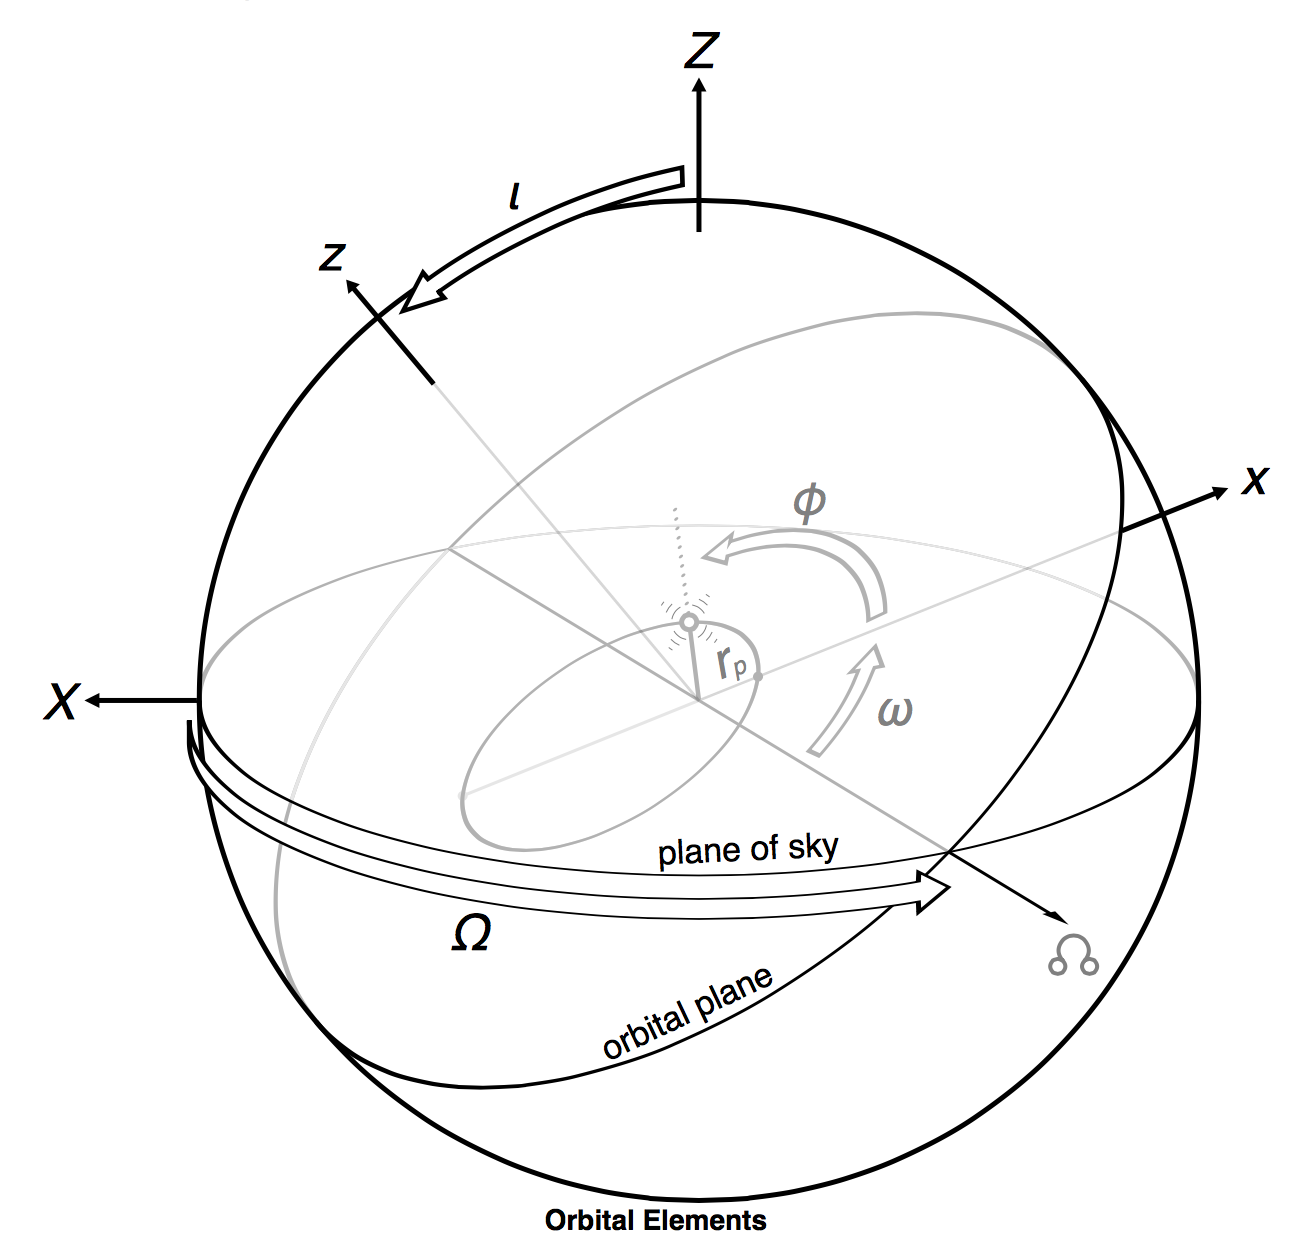
\includegraphics[width=80mm]{lalsiminspiral_orbitelements.png}
  \caption{
  \label{fig:frames} Previous LAL coordinate frames.
    \red{This diagram needs to be replaced by a new one, with the
      following changes: The $x$-axis should point along the line
      connecting the origin with body 1.  The main-text $\phiRef$ is
      the angle between line of ascending node and $\nNR$, i.e. the
      sum of the picture $\Phi+\omega$.  The mean-anomaly
      $\meanAnomaly$ in the main-text corresponds to the
      picture-symbol $\Phi$.} For the recommended default
    $\Omega=\pi/2$, the line of ascending nodes agrees with $\EyW$
    i.e. the rotation by the inclination angle $\iota$ is about the
    $\EyW$-axis.}
  \end{figure}


%%%%%%%%%%%%%%%%%%%%%%%%%%%%%%%%%%%%%%%%%%%%%%%%%%%%%%%%%%%%%%%%
\subsubsection{NR frame\boldmath$(  \ExNR, \EyNR, \EzNR)$}
%%%%%%%%%%%%%%%%%%%%%%%%%%%%%%%%%%%%%%%%%%%%%%%%%%%%%%%%%%%%%%%%

This is just a generic coordinate system, without any regards to the
concrete binary motion.  Generic coordinate systems occur in numerical
relativity, where the coordinates are chosen through same
gauge-conditions, and the binary is evolving from some initial data.
At some later time therefore, the coordinates will not have any
particular, controlled properties.

The Cartesian basis-vectors are denoted
\begin{equation}
  \ExNR, \EyNR, \EzNR.
\end{equation}
From these, spherical basis-vectors can be computed as usual
\begin{subequations}
  \label{eq:NRspherical}
\begin{align}
  \ErNR & = \cos\pNR\sin\tNR\;\ExNR + \sin\pNR\sin\tNR\;\EyNR +\cos\tNR\;\EzNR\\
  \EtNR & = \cos\pNR\cos\tNR\;\ExNR + \sin\pNR\cos\tNR\;\EyNR -\sin\tNR\;\EzNR\\
  \EpNR & =        -\sin\pNR\;\ExNR +         \cos\pNR\;\EyNR.
\end{align}
\end{subequations}

NR data is assumed to be given in spherical-harmonic modes of the
NR coordinates, as defined in the NINJA data-formats
document~\cite{Brown:2007jx}:
\begin{subequations}\label{eq:hNR}
\begin{align}
  \hpNR(\tGW) & = \frac{1}{2}\left(\EtNR_i\EtNR_j-\EpNR_i\EpNR_j\right)h^{ij}(\tGW)\\
  \hcNR(\tGW) & = \frac{1}{2}\left(\EtNR_i\EpNR_j+\EpNR_i\EtNR_j\right)h^{ij}(\tGW),
\end{align}
\end{subequations}
and
\begin{align}\label{eq:H}
  \sum_{\ell=2}^\infty\sum_{m=-\ell}^\ell H_{\ell m}&(\tGW)\;^{-2}Y_{\ell m}(\tNR,\pNR)\\
  &= \frac{r}{M}\Big(\hpNR(\tGW)-i\hcNR(\tGW)\Big).\nonumber
\end{align}
Specifically, the data-files are assumed to contain a time-series of
the $H_{\ell m}(\tGW)$ modes; given an emission direction $(\tNR,\pNR)$,
Eq.~(\ref{eq:H}) yields the GW modes $\hpNR(\tGW)$ and $\hcNR(\tGW)$, according to
the convention Eqs.~(\ref{eq:hNR}).

The gravitational wave data are given in a time-coordinate $\tGW$ of
observers at large distance.

Let us now turn to a description of the dynamics of the two bodies.
Numerical relativity defines a variety of vectors, the combination of
which defines the instantaneous state of the two bodies.  These are:
The dimensionless spin vectors of the two bodies,
\begin{equation}\label{eq:chi}
  \vec\chi_1(t),\, \vec\chi_2(t);
\end{equation}
The direction from body 2 to body 1,
\begin{equation}
  \nNR(t);
\end{equation}
the direction of the orbital angular momentum,
\begin{equation}
  \hat L(t).
\end{equation}
We do {\bf not} make any assumption about the relation of the
NR-orbital angular momentum vector $\lNR$ relative to the NR
coordinates\footnote{The customary choice of many NR groups is to
  \emph{start} NR simulations with $\lNR=\EzNR$.  Because of
  junk-radiation and precession effects, $\lNR(t)$ will deviate from
  $\EzNR$.  This deviation generally will be very small for
  aligned-spin BBH systems, but may become significant for precessing
  systems.}.
One can further define an orbital frequency
\begin{equation}\label{eq:Omega}
  \vec\Omega(t) = \nNR(t) \times \frac{d\nNR(t)}{dt}.
\end{equation}

Equations~(\ref{eq:chi})--(\ref{eq:Omega}) are defined in the
strong-field region near the black holes, and are given as a function
of the time-coordinate $t$ employed by the NR simulation in the strong
field regime.

The time-coordinates $\tGW$ and $t$ are defined at different regions
of the space-time (far-zone vs. near-zone).  Sometimes it is desirable
to relate these two time-coordinates to each other, e.g. to make a
statement about the dynamical state of the binary at the time ``when a
certain GW-frequency is reached''.  Any relation between $\tGW$ and
$t$ is ambiguous.  Often NR simulations employ an approximation of
``retarded time'', i.e.
\begin{equation}
  \label{eq:tretarted}
  \tGW = t\big|_{\rm retarted}.
\end{equation}
However, in a dynamical space-time with black holes, two difficulties
arise: First, the horizons are causally disconnected from future null
infinity, so there are no outgoing null-rays that connect the horizons
to the wave-zone.  Second, when integrating null-rays ``slightly
outside'' the horizons, the time-delay to infinity will depend on
precisely where the integration was started, as well as on the initial
direction of the null-ray.  Therefore, any relation between $\tGW$ and
$t$ should be viewed as approximate.  One should further assume that
different NR groups may use different definitions of $\tGW$ in the
data they compute.  For instance, {\tt SpEC} reports GW-waveforms
extracted at \emph{finite-radius} in terms of the NR coordinate,
$\tGW=t$, whereas extrapolated waveforms are reported using a retarded
time-coordinate with a correction of the rate of flow of time, see
Equations (7), (14a) and (14b) of Boyle \& Mroue~\cite{Boyle:2009vi}.


%%%%%%%%%%%%%%%%%%%%%%%%%%%%%%%%%%%%%%%%%%%%%%%%%%%%%%%%%%%%%%%%
\subsubsection{LAL Source-Frame \boldmath$(\ExS, \EyS, \EzS)$}
%%%%%%%%%%%%%%%%%%%%%%%%%%%%%%%%%%%%%%%%%%%%%%%%%%%%%%%%%%%%%%%%


The LAL source-frame $(\ExS, \EyS, \EzS)$ is defined as follows:
\begin{enumerate}
\item The $\EzS$-axis points along the orbital angular momentum of the binary,
  \begin{equation}\label{eq:EzS}
    \EzS\equalref \lNR.
  \end{equation}
\item The $\ExS$-axis points along the vector $\nNR$ pointing from the second
  to the first body,
  \begin{equation}\label{eq:ExS}
    \ExS\equalref\nNR.
  \end{equation}
\item The third vector $\EyS=\EzS\times\ExS$ completes the triad.
\end{enumerate}
%  \begin{equation}
%    \nNR \equalref \cos\phiRef\,\ExS + \sin\phiRef\, \EyS,
%  \end{equation}
%  where $\nNR$ is the vector pointing from body 2 in the direction of body 1.
The symbol $\equalref$ indicates that the
respective equation is only required at the reference epoch.  The
reference epoch can be unambiguously specified by a reference-time
$t_{\rm ref}$.  One can also specify a reference \emph{orbital}
frequency $\Omega_{\rm ref}$, and infer $t_{\rm ref}$ via
Eq.~(\ref{eq:Omega}), $\Omega(t_{\rm ref})=\Omega_{\rm ref}$.  If the
reference epoch is desired to be specified in terms of a
\emph{gravitational wave}--frequency, then the gravitational wave time
$\tGW$ needs to be related to the time-coordinate of the black hole
dynamics, $t$.  As discussed in the context of
Eq.~(\ref{eq:tretarted}), such an identification is ambiguous and
holds only approximately.

Equations~(\ref{eq:EzS}) and~(\ref{eq:ExS}) define the source-frame at
the reference epoch only.  They are chosen such that the
spin-components ({\tt Sx1, Sy1, Sz1}) and ({\tt S2x, S2y, S2z}) have
coordinate-invariant meaning: {\tt Sx1} is the projection of
$\vec\chi_1$ onto $\nNR$, {\tt Sz1} is the projection of $\vec\chi_1$
onto $\lNR$, etc.

The source-frame does not rotate as the binary evolves.  Specifically,
the rotation between source-frame and wave-frame described below is
constant in time.

A different reference epoch would lead to a different source-frame,
related by some rotation.  If the reference epoch is shifted by a
small amount (comparable to the orbital time-scale), $\ExS$ and $\EyS$
would rotate with the binary.  On the precession time-scale $\EzS$
would change.


The source frame has no deep intrinsic, geometric significance.  It is
merely a vehicle to describe the spin-projections onto intrinsic
geometric directions, and the basis-vectors $(\ExS, \EyS, \EzS)$ will
be convenient when writing down the transformation to the wave-frame.


%%%%%%%%%%%%%%%%%%%%%%%%%%%%%%%%
\subsubsection{Intrisinc parameters of a binary}
%%%%%%%%%%%%%%%%%%%%%%%%%%%%%%%%

Given a reference epoch, a binary is specified by the following ten
numbers:
\begin{itemize}
\item Two masses $m_1$, $m_2$.
\item Two spin-vectors $\vec\chi_1$, $\vec\chi_2$, specified through 
   the projections of the spin-vectors onto $\lNR$, $\nNR$
  and the third basis-vector (at reference time).
\item Eccentricity $e$.
\item Mean anomaly $\meanAnomaly$.  The mean anomaly is defined in terms of the current time $t$, the time of last periapsis passage $T_{\rm previous}$, and the time of next periapsis passage $T_{\rm next}$: 
\begin{equation}
\label{eq:anomaly}
\meanAnomaly=2\pi\frac{t-T_{\rm previous}}{T_{\rm next}-T_{\rm previous}}.
\end{equation}
\end{itemize}
Eccentricity should be defined somehow ``near'' the reference epoch.
A precise definition (if possible at all) is left to the future.  For
low eccentricity orbits, there is a competition between radiation
reaction driven inspiral (which results in a slightly negative average
radial velocity), and the oscillatory radial motion due to
eccentricity.  For sufficiently small eccentricity, minima in
separation may no longer exist.  If mean anomaly is still needed
despite the quite low eccentricity in such cases, one will have to
define periapsis as minimum of separation compared to a fiducial
smooth inspiral trajectory. 



%%%%%%%%%%%%%%%%%%%%%%%%%%%%%%%%%%%%%%%%%%%%%%%%%%%%%%%%%%%%%%%%
\subsubsection{Wave-Frame \boldmath$(\ExW, \EyW, \EzW)$}
\label{sec:WaveFrame}
%%%%%%%%%%%%%%%%%%%%%%%%%%%%%%%%%%%%%%%%%%%%%%%%%%%%%%%%%%%%%%%%

The wave-frame is adopted to the direction of the observer
(i.e. Earth), such that its $\EzW$-axis points toward the observer.
$\ExW$ and $\EyW$ represent basis-vectors orthogonal to the
line-of-sight, i.e. they span the plane of the sky.

The wave-frame is completely specified by three angles:
\begin{enumerate}
  \item The angle $\phiRef$ between line of ascending node and $\nNR$
    (at the reference time). \red{[In Fig.~\ref{fig:frames}, this
      angle corresponds to $\phiRef+\omega$]}
  \item The inclination $\iota$, i.e. the angle between orbital
    angular momentum $\lNR=\EzS$ and the line-of-sight $\EzW$.
  \item The angle $\Omega$ between the $\ExW$-axis and the line of
    ascending node (at the reference time).
\end{enumerate}
These three angles happen to be the Euler angles of the rotation from
wave-frame to source-frame.

The gravitational wave modes are defined as
\begin{subequations}
  \label{eq:hW}
  \begin{align}
       \hpW &= \frac{1}{2}\left(\ExW_i\ExW_j-\EyW_i\EyW_j\right)h^{ij},\\
       \hcW &= \frac{1}{2}\left(\ExW_i\EyW_j+\EyW_i\ExW_j\right)h^{ij},
  \end{align}
\end{subequations}
where the superscript 'W' indicates the LAL wave-frame.  The angle
$\Omega$ merely rotates the $\ExW$ and $\EyW$.  By definition
Eq.~(\ref{eq:hW}), this merely rotates the polarization of the GW
modes, and so $\Omega$ is fully degenerate with the GW polarization.  


%% The three angles that rotate the source-frame into to the wave-frame
%% satisfy different purposes, with different degree of impact on the
%% waveforms:

%% The inclination $\iota$ decides between edge-on and face-on view of
%% the binary, and will significantly impact the waveforms.  The phase
%% $\phiRef$ will induce a phase-shift of the waveforms, a less
%% signifcant effect.  Finally, $\Omega$ is entirely degenerate with the
%% polarization angle of the two wave polarizations.  Changing $\Omega$
%% merely rotates $\hpW$ and $\hcW$ into each other; it only determines
%% the basis of the GW polarizations.

Note that the phase-angle $\phiRef$ is specified without regard to the
location of periapsis of the binary (this differs from the previous LAL
convention).  This new definition decouples the specification of
periapsis location and the specification of orbital phase, and avoids
the ambiguity that would arise in the zero-eccentricity limit of
definitions involving periapsis. Indeed, for fixed $\phiRef$ and fixed
$\meanAnomaly$, as eccentricity approaches zero, the waveforms will
approach the identical circular form, independent of the value of
$\meanAnomaly$.




%%%%%%%%%%%%%%%%%%%%%%%%%%%%%%%%%%%%%%%%%%%%%%%%%%%%%%%%%%%%%%%%
\subsection{Relationship between frames}
\label{sec:Relations}
%%%%%%%%%%%%%%%%%%%%%%%%%%%%%%%%%%%%%%%%%%%%%%%%%%%%%%%%%%%%%%%%

\subsubsection{From source-frame to wave-frame}

The relation between source-frame and wave-frame can be easily derived
following the three rotations that rotate one into the other frame:


Beginning in the source-frame, $\ExS, \EyS, \EzS$, we first apply the rotation
by $\phiRef$ around $\EzS$, which yields a frame with basis-vectors $\hat p, \hat q, \EzS$:
\begin{subequations}
  \label{eq:phiRef-Rotation1}
\begin{align}
  \hat p &= \cos\phiRef\,\ExS - \sin\phiRef\,\EyS,\\
  \hat q &= \sin\phiRef\,\ExS+\cos\phiRef\,\EyS,\\
  \EzS & = \EzS.
\end{align}
\end{subequations}
The inverse rotation is
\begin{subequations}
  \label{eq:phiRef-Rotation2}
\begin{align}
  \ExS &= \;\;\;\cos\phiRef\,\hat p + \sin\phiRef\,\hat q,\\
  \EyS &= -\sin\phiRef\,\hat p+\cos\phiRef\,\hat q,\\
  \EzS & = \EzS.
\end{align}
\end{subequations}
The vectors $\hat p, \hat q$ form an orthonormal basis of the
$\ExS$-$\EyS$ plane, such that $\hat p$ points in the direction of
ascending node.


Next, we rotate around the line of ascending node by the inclination $\iota$,
resulting in basis-vectors
\begin{subequations}
  \label{eq:iota-Rotation1}
\begin{align}
  \hat P&=\hat p,\\
  \hat Q&=\cos\iota\,\hat q - \sin\iota\,\EzS,\\
  \hat Z&=\sin\iota\,\hat q+\cos\iota\,\EzS.
\end{align}
\end{subequations}
 $\hat P$ and $\hat Q$ form an orthonormal basis of the $\ExW$-$\EyW$
plane with $\hat P$ pointing in the direction of ascending node.
The inverse rotation is
\begin{subequations}
  \label{eq:iota-Rotation2}
\begin{align}
  \hat p&=\hat P,\\
  \hat q&=\;\;\;\cos\iota\,\hat Q + \sin\iota\,\EzW,\\
  \EzS &=-\sin\iota\,\hat Q+\cos\iota\,\EzW.
\end{align}
\end{subequations}


The final rotation rotates $\hat P$ and $\hat Q$
around $\EzW$ into $\ExW,\EyW$:
\begin{subequations}
  \label{eq:Omega-Rotation1}
\begin{align}
  \ExW&=\cos\Omega\,\hat P-\sin\Omega\,\hat Q,\\
  \EyW&=\sin\Omega\,\hat P+\cos\Omega\,\hat Q,\\
  \EzW&=\EzW.
\end{align}
\end{subequations}
The inverse rotation is
\begin{subequations}
  \label{eq:Omega-Rotation2}
\begin{align}
  \hat P&=\;\;\;\cos\Omega\,\ExW+\sin\Omega\,\EyW,\\
  \hat Q&=-\sin\Omega\,\ExW+\cos\Omega\,\EyW,\\
  \EzW&=\EzW.
\end{align}
\end{subequations}

Substituting Eqs.~(\ref{eq:phiRef-Rotation1}),~(\ref{eq:iota-Rotation1}) and~(\ref{eq:Omega-Rotation1}) into each other, one obtains the entire transformation:
\begin{subequations}
  \label{eq:Source-To-Wave}
  \begin{align}
    \ExW=& \left(\cos\Omega\cos\phiRef-\sin\Omega\cos\iota\sin\phiRef\right)\ExS
    \nonumber \\
    & + \left(-\cos\Omega\sin\phiRef-\sin\Omega\cos\iota\cos\phiRef\right)\EyS
    \nonumber\\
    & + \sin\Omega\sin\iota\,\EzS,\\
\EyW=& \left(\sin\Omega\cos\phiRef+\cos\Omega\cos\iota\sin\phiRef\right)\ExS
    \nonumber \\
    & + \left(-\sin\Omega\sin\phiRef+\cos\Omega\cos\iota\cos\phiRef\right)\EyS
    \nonumber\\
    & - \cos\Omega\sin\iota\,\EzS,\\
\label{eq:Z_from_z}
\EzW=&\sin\iota\sin\phiRef\,\ExS+\sin\iota\cos\phiRef\,\EyS + \cos\iota\,\EzS.
  \end{align}
  \end{subequations}


The inverse transformation is obtained from
Eqs.~(\ref{eq:phiRef-Rotation2}), (\ref{eq:iota-Rotation2})
and~(\ref{eq:Omega-Rotation2}):
\begin{subequations}
  \label{eq:Wave-To-Source}
  \begin{align}
    \ExS=& \left(\cos\Omega\cos\phiRef-\sin\Omega\cos\iota\sin\phiRef\right)\ExW
    \nonumber \\
    & + \left(\sin\Omega\cos\phiRef+\cos\Omega\cos\iota\sin\phiRef\right)\EyW
    \nonumber\\
    & + \sin\iota\sin\phiRef\,\EzW,\\
\EyS=& \left(-\cos\Omega\sin\phiRef-\sin\Omega\cos\iota\cos\phiRef\right)\ExW
    \nonumber \\
    & + \left(-\sin\Omega\sin\phiRef+\cos\Omega\cos\iota\cos\phiRef\right)\EyW
    \nonumber\\
    & + \sin\iota\cos\phiRef\,\EzW,\\
\label{eq:z_from_Z}
    \EzS=&\sin\Omega\sin\iota\,\ExW-\cos\Omega\sin\iota\,\EyW + \cos\iota\,\EzW.
  \end{align}
  \end{subequations}
Equation~(\ref{eq:z_from_Z}) shows that $\Omega$ determines the
direction of $\lNR=\hat z$ on the plane of the sky.  For $\Omega=0$,
$\lNR$ lies in the $\EyW$-$\EzW$ plane, and for $\Omega=\pi/2$, it lies
in the $\ExW$-$\EzW$ plane.

This latter choice ($\Omega=\pi/2$) is already respected by many LAL
waveform models.  Therefore, in the absence of a reason to do
otherwise, all waveform models should default to $\Omega=\pi/2$.  

With this recommended default $\Omega=\pi/2$,
Eqs.~(\ref{eq:Source-To-Wave}) simplify to
\begin{subequations}
  \label{eq:Source-To-Wave-Omega0}
  \begin{align}
    \ExW=& -\cos\iota\sin\phiRef\,\ExS-\cos\iota\cos\phiRef\,\EyS\,+\sin\iota\,\EzS,\\
    \EyW=&\quad\quad\;\;\; \cos\phiRef\,\ExS\qquad\,-\sin\phiRef\,\EyS,\\
\label{eq:Z_from_z-Omega0}
\EzW=&\;\;\;\;\,\sin\iota\sin\phiRef\,\ExS+\sin\iota\cos\phiRef\,\EyS\, + \cos\iota\,\EzS.
  \end{align}
  \end{subequations}
The inverse transformation (\ref{eq:Wave-To-Source}) simplifies to 
\begin{subequations}
  \label{eq:Wave-To-Source-Omega0}
  \begin{align}
    \ExS=& -\cos\iota\sin\phiRef\,\ExW+\cos\phiRef\,\EyW
    + \sin\iota\sin\phiRef\,\EzW,\\
    \EyS=& -\cos\iota\cos\phiRef\,\ExW-\sin\phiRef\,\EyW
    + \sin\iota\cos\phiRef\,\EzW,\\
    \EzS=&\qquad\quad\;\,\sin\iota\,\ExW \qquad\qquad\qquad\;+\cos\iota\,\EzW.
  \end{align}
  \end{subequations}


%%%%%%%%%%%%%%%%%%%%%%%%%%%%%%%%%%%%%%%%%%%%%%%%%%%%%%%%%%%%%%%%
\subsubsection{From NR-frame to wave-frame}
%%%%%%%%%%%%%%%%%%%%%%%%%%%%%%%%%%%%%%%%%%%%%%%%%%%%%%%%%%%%%%%%


Equations~(\ref{eq:Source-To-Wave}) and
(\ref{eq:Source-To-Wave-Omega0}) are of particular importance.  By
definition, the source-frame basis-vectors are trivially related to
vectorial quantities of the CBC dynamics:
\begin{subequations}
  \begin{align}
    \ExS&\equalref \nNR,\\
    \EyS&\equalref (\lNR\times\nNR),\\
    \EzS&\equalref \lNR.
  \end{align}
\end{subequations}
Therefore, if the dynamics vectors $\lNR$ and $\nNR$ are known in any
coordinate system ---e.g., the NR coordinates--- then
Eqs.~(\ref{eq:Source-To-Wave}) yield the wave-frame basis-vectors in those
coordinates.  Specifically, for $\Omega=\pi/2$,
Eqs.~(\ref{eq:Source-To-Wave-Omega0}) yield
\begin{subequations}
  \begin{align}
    \ExW &\equalref-\cos\iota\left[\sin\phiRef\,\nNR +\cos\phiRef\,\lNR\times\nNR\right]+\sin\iota\lNR,\\
    \EyW &\equalref \qquad\quad\;\,\cos\phiRef\,\nNR -\sin\phiRef\,\lNR\times\nNR,\\
\label{eq:Z}
    \EzW&\equalref\;\;\;\; \sin i\left[\sin\phiRef\,\nNR +\cos\phiRef\,\lNR\times\nNR\right]
    +\cos i\,\lNR.
  \end{align}
\end{subequations}

Let us consider next the transformation of the GW strain polarizations
from the generic (NR) frame Eq.~(\ref{eq:NRspherical}) to the
wave-frame.  $\ExW$ and $\EyW$ are orthogonal to the direction of
propagation $\EzW=\ErNR$ of the gravitational wave.  Therefore,
$(\EtNR, \EpNR)$ can be rotated into $(\ExW, \EyW)$ through a rotation
by an angle $\alpha$:
\begin{subequations}\label{eq:alpha}
\begin{align}
\ExW & = \cos\alpha\,\EtNR - \sin\alpha\,\EpNR,\\
\label{eq:alphaY}
\EyW & = \sin\alpha\,\EtNR +\cos\alpha\,\EpNR.
\end{align}
\end{subequations}
Substituting Eqs.~(\ref{eq:alpha}) into Eqs.~(\ref{eq:hW}) we can compute $\hpW$ and $\hcW$ in terms of $(\EtNR,\EpNR)$.  Comparing further with Eqs.~(\ref{eq:hNR}), we find:
\begin{subequations}
\label{eq:PolarizationTrafo}
\begin{align}
  \hpW(\tGW) &= \cos\left(2\alpha\right)\,\hpNR(\tGW) -\sin\left(2\alpha\right)\,\hcNR(\tGW),\\
  \hcW(\tGW) &= \sin(2\alpha)\,\hpNR(\tGW)+\cos\left(2\alpha\right)\,\hcNR(\tGW).
\end{align}
\end{subequations}
Not surprising, the GW polarizations in the wave-frame are obtained
from those in the NR-frame by a rotation of $2\alpha$.

The wave-frame $\ExW, \EyW$ depend on $\Omega$, and therefore $\hpW$
and $\hcW$ also depend on $\Omega$.  We can make this dependence
explicit by resorting to the intermediate vectors $\hat P$ and
$\hat Q$.  These are also orthogonal to $\EzW$, therefore they, too,
can be obtained from $\EtNR$ and $\EpNR$ by a rotation:
\begin{subequations}
\begin{align}
\hat P & = \cos\alpha'\,\EtNR - \sin\alpha'\,\EpNR,\\
\hat Q & = \sin\alpha'\,\EtNR + \cos\alpha'\,\EpNR.
\end{align}
\end{subequations}
However, $\hat P$ and $\hat Q$ are independent of $\Omega$ and
therefore, $\alpha'$ is independent of $\Omega$.  Because
$(\ExW, \EyW)$ are rotated by $\Omega$ relative to $(\hat P, \hat Q)$,
we have
\begin{equation}
\alpha = \Omega+\alpha'.
\end{equation}
Because rotations add, we can therefore write
\begin{equation}\label{eq:polarization-rotation}
\left(\begin{aligned}\hpW\\\hcW \end{aligned}\right)
= {\mathbf R}_{2\Omega}\; {\mathbf R}_{2\alpha'} 
\left(\begin{aligned}\hpNR\\\hcNR \end{aligned}\right),
\end{equation}
where ${\mathbf R}_\beta$ denotes a 2x2 rotation matrix,
\begin{equation}
{\mathbf R}_\beta = \left(\begin{aligned}&\cos\beta & -\sin\beta \\ & \sin\beta & \cos\beta\end{aligned}\right).
\end{equation}

Equation~(\ref{eq:polarization-rotation}) thus implies that the
waveform-modes are obtained from the NR-polarizations by (i) applying
an $\Omega$-independent rotation by $2\alpha'$; followed by (ii) a
rotation by $2\Omega$.

For $\Omega=\pi/2$, we have ${\mathbf R}_\pi = -{\mathbf 1}$.
Therefore, between $\Omega=0$ [inclination rotated about X-axis] and
$\Omega=\pi/2$ [inclination rotated about Y-axis], the waveform
polarization pick up precisely an overall minus-sign. 


%%%%%%%%%%%%%%%%%%%%%%%%%%%%%%%%%%%%%%%%%%%%%%%%%%%%%%%%%%%%%%%%
\subsection{Computing GW polarizations in the LAL wave-frame}
\label{sec:NR-LAL-Trafo}
%%%%%%%%%%%%%%%%%%%%%%%%%%%%%%%%%%%%%%%%%%%%%%%%%%%%%%%%%%%%%%%%

Let us finally write down explicit instructions of how to obtain GW
polarizations in LAL convention, given NR waveform data.  
Given parameters {\tt i, phiRef} passed into {\tt
  XLALSimInspiralChooseTDWaveform}, proceed as follows:

\begin{enumerate}
\item Define $\phiRef=\mbox{phiRef}$, $\iota={\tt i}$.
\item Compute $\EzW_{\rm ref}$ at the reference time by evaluating Eq.~(\ref{eq:Z}).
%\footnote{Note that Eq.~(\ref{eq:Z}) is valid for any value of $\Omega$, because the original Eq.~(\ref{eq:Z_from_z}) is indepenedent of $\Omega$.}.
\item Because $\EzW$ points in the direction of emission of the
gravitational wave, we must have
\begin{equation}
  \EzW_{\rm ref} \equalref
  \left(\begin{gathered}
    \cos\pNR\sin\tNR\\
    \sin\pNR\sin\tNR\\
    \cos\tNR\end{gathered}
    \right).
\end{equation}
From this equality, read off $(\tNR, \pNR)$.  Then compute the
NR-basis vectors $\EtNR, \EpNR$ from Eqs.~(\ref{eq:NRspherical}).
\item If $\Omega=\pi/2$, compute $\sin\alpha$ and $\cos\alpha$ by taking inner products
  of Eq.~(\ref{eq:alphaY}) with $\EtNR$ and $\EpNR$:
  \begin{subequations}
  \begin{align}
    \sin\alpha& = \cos\phiRef\,\nNR\cdot\EtNR- \sin\phiRef\,(\lNR\times\nNR)\cdot\EtNR,\\
    \cos\alpha& = \cos\phiRef\,\nNR\cdot\EpNR - \sin\phiRef\,(\lNR\times\nNR)\cdot\EpNR.
  \end{align}
\end{subequations}
  If $\Omega\neq \pi/2$, compute instead inner products based on
  Eqs.~(\ref{eq:Source-To-Wave}).
\item Substitute $(\tNR, \pNR)$ into Eqs.~(\ref{eq:H})
  and~(\ref{eq:hNR}) to compute $\hpNR(\tGW)$ and $\hcNR(\tGW)$.
\item Compute $\cos 2\alpha=\cos^2\alpha\!-\!\sin^2\alpha$ and $\sin 2\alpha=2\cos\alpha\sin\alpha$.  Substitute into Eqs.~(\ref{eq:PolarizationTrafo}) to compute $\hpW(\tGW)$ and $\hcW(\tGW)$.
\end{enumerate}


%%%%%%%%%%%%%%%%%%%%%%%%%%%%%%%%%%%%%%%%%%%%%%%%%%%%%%%%%%%%%%%%
\subsubsection{Evaluate spin-consistency in LAL source-frame}
%%%%%%%%%%%%%%%%%%%%%%%%%%%%%%%%%%%%%%%%%%%%%%%%%%%%%%%%%%%%%%%%

The parameters {\tt S1x, S1y, S1z, S2x, S2y,S2z} passed into {\tt
  LALSimInspiralChooseTDwaveform} are supposed to be the LAL
source-frame parameters, i.e. these parameters should simply be the
projections of $\vec\chi_{1,2}$ onto the source-frame basis-vectors
$(\ExS,\EyS,\EzS)$.  Substituting Eqs.~(\ref{eq:EzS}) and (\ref{eq:ExS}),
one arrives at the following consistency conditions:
\begin{subequations}
\label{eq:SpinConsistency}
  \begin{align}
    \mbox{\tt S1x} &  \equalref \vec\chi_1 \cdot \nNR,\\
    \mbox{\tt S1y} &  \equalref \vec\chi_1\cdot (\lNR\times\nNR),\\
    \mbox{\tt S1z} &  \equalref \vec\chi_1 \cdot \lNR.
  \end{align}
\end{subequations}
The conditions for body 2 are obtained by $1\leftrightarrow 2$.\\

%%%%%%%%%%%%%%%%%%%%%%%%%%%%%%%%%%%%%%%%%%%%%%%%%%%%%%%%%%%%%%%%

%%%%%%%%%%
\section{Discussion}
\label{sec:discussion}
%%%%%%%%%%

With this new infrastructure it is very easy and much less memory intensive to use NR waveforms
directly for data-analysis applications. The ``NR\_hdf5'' approximant works much the same as any other approximant
in lalsimulation, but there are a few important differences.
The user must supply the location of the HDF5 file, a functionality which was already implemented for NINJA, but was not
previously used in lalsimulation. Secondly, the user must be careful to supply the mass ratio and spin values that
are consistent with the NR files, and the spin values have to be specified in the LAL source frame (see Eqn. (\ref{eq:SpinConsistency})). \\

The current implementation still suffers from a few caveats and drawbacks. As opposed to the continuous waveform approximants, at the moment the metadata are only referring to the beginning of the waveform and not some reference time, which can be chosen freely. While this is not a problem for aligned-spin binaries, this is a big concern for precessing simulations since various quantities, in particular the spins and the orbital angular momentum, are time-dependent. To fully integrate this desired freedom, additional information needs to be incorporated into the HDF5 files and the waveform generator functions accordingly. In the future, we plan to include the frequency evolution of the spins and the orbital angular momentum.

%%%%%%%%%%%%%%%%%%%%%%%%%Acknowledgements%%%%%%%%%%%%%%%%%%%%
\section*{Acknowledgements}
We thank Kent Blackburn for carefully reading through the manuscript and providing useful comments.
Many thanks for discussions regarding the frame coordinate transformations to Stas Babak, Jolien Creighton, Michael P\"urrer and Ricardo Sturani.
%%%%%%%%%%%%%%%%%%%%%%%%%Appendices%%%%%%%%%%%%%%%%%%%%%%%%

%%%%%References%%%%%%%%%%%%%%%%%

\bibliography{nrinj}

%%%%%%%%%%
\end{document}
%%%%%%%%%%
